% This file was created by matplotlib2tikz v0.6.0.
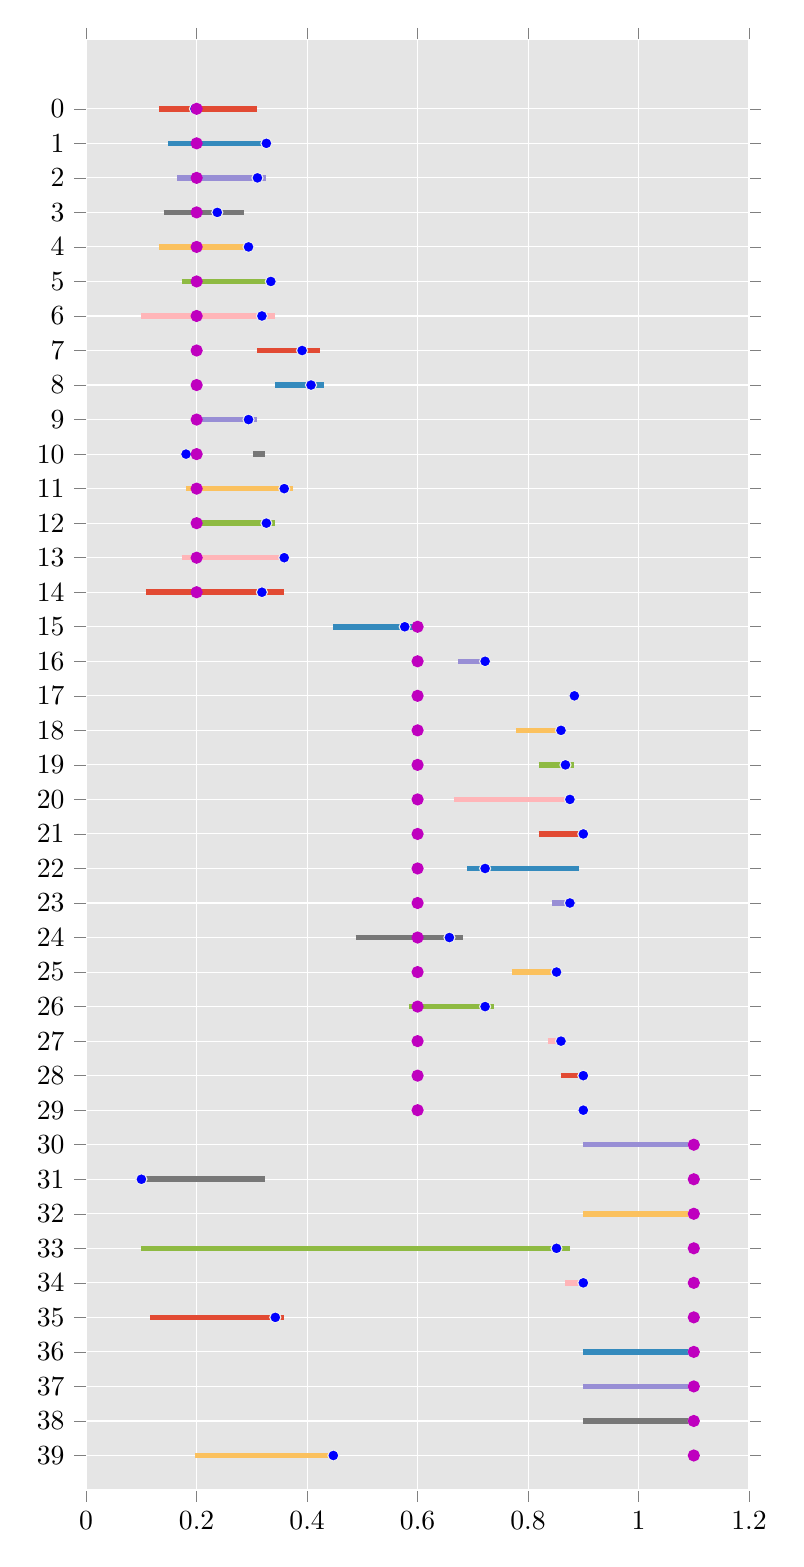
\begin{tikzpicture}

\definecolor{color6}{rgb}{1,0.709803921568627,0.72156862745098}
\definecolor{color4}{rgb}{0.984313725490196,0.756862745098039,0.368627450980392}
\definecolor{color0}{rgb}{0.75,0,0.75}
\definecolor{color3}{rgb}{0.596078431372549,0.556862745098039,0.835294117647059}
\definecolor{color1}{rgb}{0.886274509803922,0.290196078431373,0.2}
\definecolor{color5}{rgb}{0.556862745098039,0.729411764705882,0.258823529411765}
\definecolor{color2}{rgb}{0.203921568627451,0.541176470588235,0.741176470588235}

\begin{axis}[
xmin=0, xmax=1.2,
ymin=-1, ymax=41,
width=10cm,
height=20cm,
ytick={0,1,2,3,4,5,6,7,8,9,10,11,12,13,14,15,16,17,18,19,20,21,22,23,24,25,26,27,28,29,30,31,32,33,34,35,36,37,38,39},
yticklabels={39,38,37,36,35,34,33,32,31,30,29,28,27,26,25,24,23,22,21,20,19,18,17,16,15,14,13,12,11,10,9,8,7,6,5,4,3,2,1,0},
tick align=outside,
xmajorgrids,
x grid style={white},
ymajorgrids,
y grid style={white},
axis line style={white},
axis background/.style={fill=white!89.803921568627459!black}
]
\addplot [only marks, draw=white!93.333333333333329!black, fill=blue, colormap={mymap}{[1pt]
  rgb(0pt)=(0,0,0.5);
  rgb(22pt)=(0,0,1);
  rgb(25pt)=(0,0,1);
  rgb(68pt)=(0,0.86,1);
  rgb(70pt)=(0,0.9,0.967741935483871);
  rgb(75pt)=(0.0806451612903226,1,0.887096774193548);
  rgb(128pt)=(0.935483870967742,1,0.0322580645161291);
  rgb(130pt)=(0.967741935483871,0.962962962962963,0);
  rgb(132pt)=(1,0.925925925925926,0);
  rgb(178pt)=(1,0.0740740740740741,0);
  rgb(182pt)=(0.909090909090909,0,0);
  rgb(200pt)=(0.5,0,0)
}, visualization depends on={\thisrow{sizedata} \as\perpointmarksize}, scatter/@pre marker code/.append style={/tikz/mark size=\perpointmarksize}]
table {%
x                      y                      sizedata
+1.969696969696970e-01 +3.900000000000000e+01 +5.641895835477563e+00
};
\addplot [only marks, draw=color0, fill=color0, colormap={mymap}{[1pt]
  rgb(0pt)=(0,0,0.5);
  rgb(22pt)=(0,0,1);
  rgb(25pt)=(0,0,1);
  rgb(68pt)=(0,0.86,1);
  rgb(70pt)=(0,0.9,0.967741935483871);
  rgb(75pt)=(0.0806451612903226,1,0.887096774193548);
  rgb(128pt)=(0.935483870967742,1,0.0322580645161291);
  rgb(130pt)=(0.967741935483871,0.962962962962963,0);
  rgb(132pt)=(1,0.925925925925926,0);
  rgb(178pt)=(1,0.0740740740740741,0);
  rgb(182pt)=(0.909090909090909,0,0);
  rgb(200pt)=(0.5,0,0)
}, visualization depends on={\thisrow{sizedata} \as\perpointmarksize}, scatter/@pre marker code/.append style={/tikz/mark size=\perpointmarksize}]
table {%
x                      y                      sizedata
+2.000000000000000e-01 +3.900000000000000e+01 +5.641895835477563e+00
};
\addplot [only marks, draw=white!93.333333333333329!black, fill=blue, colormap={mymap}{[1pt]
  rgb(0pt)=(0,0,0.5);
  rgb(22pt)=(0,0,1);
  rgb(25pt)=(0,0,1);
  rgb(68pt)=(0,0.86,1);
  rgb(70pt)=(0,0.9,0.967741935483871);
  rgb(75pt)=(0.0806451612903226,1,0.887096774193548);
  rgb(128pt)=(0.935483870967742,1,0.0322580645161291);
  rgb(130pt)=(0.967741935483871,0.962962962962963,0);
  rgb(132pt)=(1,0.925925925925926,0);
  rgb(178pt)=(1,0.0740740740740741,0);
  rgb(182pt)=(0.909090909090909,0,0);
  rgb(200pt)=(0.5,0,0)
}, visualization depends on={\thisrow{sizedata} \as\perpointmarksize}, scatter/@pre marker code/.append style={/tikz/mark size=\perpointmarksize}]
table {%
x                      y                      sizedata
+3.262626262626263e-01 +3.800000000000000e+01 +5.641895835477563e+00
};
\addplot [only marks, draw=color0, fill=color0, colormap={mymap}{[1pt]
  rgb(0pt)=(0,0,0.5);
  rgb(22pt)=(0,0,1);
  rgb(25pt)=(0,0,1);
  rgb(68pt)=(0,0.86,1);
  rgb(70pt)=(0,0.9,0.967741935483871);
  rgb(75pt)=(0.0806451612903226,1,0.887096774193548);
  rgb(128pt)=(0.935483870967742,1,0.0322580645161291);
  rgb(130pt)=(0.967741935483871,0.962962962962963,0);
  rgb(132pt)=(1,0.925925925925926,0);
  rgb(178pt)=(1,0.0740740740740741,0);
  rgb(182pt)=(0.909090909090909,0,0);
  rgb(200pt)=(0.5,0,0)
}, visualization depends on={\thisrow{sizedata} \as\perpointmarksize}, scatter/@pre marker code/.append style={/tikz/mark size=\perpointmarksize}]
table {%
x                      y                      sizedata
+2.000000000000000e-01 +3.800000000000000e+01 +5.641895835477563e+00
};
\addplot [only marks, draw=white!93.333333333333329!black, fill=blue, colormap={mymap}{[1pt]
  rgb(0pt)=(0,0,0.5);
  rgb(22pt)=(0,0,1);
  rgb(25pt)=(0,0,1);
  rgb(68pt)=(0,0.86,1);
  rgb(70pt)=(0,0.9,0.967741935483871);
  rgb(75pt)=(0.0806451612903226,1,0.887096774193548);
  rgb(128pt)=(0.935483870967742,1,0.0322580645161291);
  rgb(130pt)=(0.967741935483871,0.962962962962963,0);
  rgb(132pt)=(1,0.925925925925926,0);
  rgb(178pt)=(1,0.0740740740740741,0);
  rgb(182pt)=(0.909090909090909,0,0);
  rgb(200pt)=(0.5,0,0)
}, visualization depends on={\thisrow{sizedata} \as\perpointmarksize}, scatter/@pre marker code/.append style={/tikz/mark size=\perpointmarksize}]
table {%
x                      y                      sizedata
+3.101010101010101e-01 +3.700000000000000e+01 +5.641895835477563e+00
};
\addplot [only marks, draw=color0, fill=color0, colormap={mymap}{[1pt]
  rgb(0pt)=(0,0,0.5);
  rgb(22pt)=(0,0,1);
  rgb(25pt)=(0,0,1);
  rgb(68pt)=(0,0.86,1);
  rgb(70pt)=(0,0.9,0.967741935483871);
  rgb(75pt)=(0.0806451612903226,1,0.887096774193548);
  rgb(128pt)=(0.935483870967742,1,0.0322580645161291);
  rgb(130pt)=(0.967741935483871,0.962962962962963,0);
  rgb(132pt)=(1,0.925925925925926,0);
  rgb(178pt)=(1,0.0740740740740741,0);
  rgb(182pt)=(0.909090909090909,0,0);
  rgb(200pt)=(0.5,0,0)
}, visualization depends on={\thisrow{sizedata} \as\perpointmarksize}, scatter/@pre marker code/.append style={/tikz/mark size=\perpointmarksize}]
table {%
x                      y                      sizedata
+2.000000000000000e-01 +3.700000000000000e+01 +5.641895835477563e+00
};
\addplot [only marks, draw=white!93.333333333333329!black, fill=blue, colormap={mymap}{[1pt]
  rgb(0pt)=(0,0,0.5);
  rgb(22pt)=(0,0,1);
  rgb(25pt)=(0,0,1);
  rgb(68pt)=(0,0.86,1);
  rgb(70pt)=(0,0.9,0.967741935483871);
  rgb(75pt)=(0.0806451612903226,1,0.887096774193548);
  rgb(128pt)=(0.935483870967742,1,0.0322580645161291);
  rgb(130pt)=(0.967741935483871,0.962962962962963,0);
  rgb(132pt)=(1,0.925925925925926,0);
  rgb(178pt)=(1,0.0740740740740741,0);
  rgb(182pt)=(0.909090909090909,0,0);
  rgb(200pt)=(0.5,0,0)
}, visualization depends on={\thisrow{sizedata} \as\perpointmarksize}, scatter/@pre marker code/.append style={/tikz/mark size=\perpointmarksize}]
table {%
x                      y                      sizedata
+2.373737373737374e-01 +3.600000000000000e+01 +5.641895835477563e+00
};
\addplot [only marks, draw=color0, fill=color0, colormap={mymap}{[1pt]
  rgb(0pt)=(0,0,0.5);
  rgb(22pt)=(0,0,1);
  rgb(25pt)=(0,0,1);
  rgb(68pt)=(0,0.86,1);
  rgb(70pt)=(0,0.9,0.967741935483871);
  rgb(75pt)=(0.0806451612903226,1,0.887096774193548);
  rgb(128pt)=(0.935483870967742,1,0.0322580645161291);
  rgb(130pt)=(0.967741935483871,0.962962962962963,0);
  rgb(132pt)=(1,0.925925925925926,0);
  rgb(178pt)=(1,0.0740740740740741,0);
  rgb(182pt)=(0.909090909090909,0,0);
  rgb(200pt)=(0.5,0,0)
}, visualization depends on={\thisrow{sizedata} \as\perpointmarksize}, scatter/@pre marker code/.append style={/tikz/mark size=\perpointmarksize}]
table {%
x                      y                      sizedata
+2.000000000000000e-01 +3.600000000000000e+01 +5.641895835477563e+00
};
\addplot [only marks, draw=white!93.333333333333329!black, fill=blue, colormap={mymap}{[1pt]
  rgb(0pt)=(0,0,0.5);
  rgb(22pt)=(0,0,1);
  rgb(25pt)=(0,0,1);
  rgb(68pt)=(0,0.86,1);
  rgb(70pt)=(0,0.9,0.967741935483871);
  rgb(75pt)=(0.0806451612903226,1,0.887096774193548);
  rgb(128pt)=(0.935483870967742,1,0.0322580645161291);
  rgb(130pt)=(0.967741935483871,0.962962962962963,0);
  rgb(132pt)=(1,0.925925925925926,0);
  rgb(178pt)=(1,0.0740740740740741,0);
  rgb(182pt)=(0.909090909090909,0,0);
  rgb(200pt)=(0.5,0,0)
}, visualization depends on={\thisrow{sizedata} \as\perpointmarksize}, scatter/@pre marker code/.append style={/tikz/mark size=\perpointmarksize}]
table {%
x                      y                      sizedata
+2.939393939393939e-01 +3.500000000000000e+01 +5.641895835477563e+00
};
\addplot [only marks, draw=color0, fill=color0, colormap={mymap}{[1pt]
  rgb(0pt)=(0,0,0.5);
  rgb(22pt)=(0,0,1);
  rgb(25pt)=(0,0,1);
  rgb(68pt)=(0,0.86,1);
  rgb(70pt)=(0,0.9,0.967741935483871);
  rgb(75pt)=(0.0806451612903226,1,0.887096774193548);
  rgb(128pt)=(0.935483870967742,1,0.0322580645161291);
  rgb(130pt)=(0.967741935483871,0.962962962962963,0);
  rgb(132pt)=(1,0.925925925925926,0);
  rgb(178pt)=(1,0.0740740740740741,0);
  rgb(182pt)=(0.909090909090909,0,0);
  rgb(200pt)=(0.5,0,0)
}, visualization depends on={\thisrow{sizedata} \as\perpointmarksize}, scatter/@pre marker code/.append style={/tikz/mark size=\perpointmarksize}]
table {%
x                      y                      sizedata
+2.000000000000000e-01 +3.500000000000000e+01 +5.641895835477563e+00
};
\addplot [only marks, draw=white!93.333333333333329!black, fill=blue, colormap={mymap}{[1pt]
  rgb(0pt)=(0,0,0.5);
  rgb(22pt)=(0,0,1);
  rgb(25pt)=(0,0,1);
  rgb(68pt)=(0,0.86,1);
  rgb(70pt)=(0,0.9,0.967741935483871);
  rgb(75pt)=(0.0806451612903226,1,0.887096774193548);
  rgb(128pt)=(0.935483870967742,1,0.0322580645161291);
  rgb(130pt)=(0.967741935483871,0.962962962962963,0);
  rgb(132pt)=(1,0.925925925925926,0);
  rgb(178pt)=(1,0.0740740740740741,0);
  rgb(182pt)=(0.909090909090909,0,0);
  rgb(200pt)=(0.5,0,0)
}, visualization depends on={\thisrow{sizedata} \as\perpointmarksize}, scatter/@pre marker code/.append style={/tikz/mark size=\perpointmarksize}]
table {%
x                      y                      sizedata
+3.343434343434344e-01 +3.400000000000000e+01 +5.641895835477563e+00
};
\addplot [only marks, draw=color0, fill=color0, colormap={mymap}{[1pt]
  rgb(0pt)=(0,0,0.5);
  rgb(22pt)=(0,0,1);
  rgb(25pt)=(0,0,1);
  rgb(68pt)=(0,0.86,1);
  rgb(70pt)=(0,0.9,0.967741935483871);
  rgb(75pt)=(0.0806451612903226,1,0.887096774193548);
  rgb(128pt)=(0.935483870967742,1,0.0322580645161291);
  rgb(130pt)=(0.967741935483871,0.962962962962963,0);
  rgb(132pt)=(1,0.925925925925926,0);
  rgb(178pt)=(1,0.0740740740740741,0);
  rgb(182pt)=(0.909090909090909,0,0);
  rgb(200pt)=(0.5,0,0)
}, visualization depends on={\thisrow{sizedata} \as\perpointmarksize}, scatter/@pre marker code/.append style={/tikz/mark size=\perpointmarksize}]
table {%
x                      y                      sizedata
+2.000000000000000e-01 +3.400000000000000e+01 +5.641895835477563e+00
};
\addplot [only marks, draw=white!93.333333333333329!black, fill=blue, colormap={mymap}{[1pt]
  rgb(0pt)=(0,0,0.5);
  rgb(22pt)=(0,0,1);
  rgb(25pt)=(0,0,1);
  rgb(68pt)=(0,0.86,1);
  rgb(70pt)=(0,0.9,0.967741935483871);
  rgb(75pt)=(0.0806451612903226,1,0.887096774193548);
  rgb(128pt)=(0.935483870967742,1,0.0322580645161291);
  rgb(130pt)=(0.967741935483871,0.962962962962963,0);
  rgb(132pt)=(1,0.925925925925926,0);
  rgb(178pt)=(1,0.0740740740740741,0);
  rgb(182pt)=(0.909090909090909,0,0);
  rgb(200pt)=(0.5,0,0)
}, visualization depends on={\thisrow{sizedata} \as\perpointmarksize}, scatter/@pre marker code/.append style={/tikz/mark size=\perpointmarksize}]
table {%
x                      y                      sizedata
+3.181818181818182e-01 +3.300000000000000e+01 +5.641895835477563e+00
};
\addplot [only marks, draw=color0, fill=color0, colormap={mymap}{[1pt]
  rgb(0pt)=(0,0,0.5);
  rgb(22pt)=(0,0,1);
  rgb(25pt)=(0,0,1);
  rgb(68pt)=(0,0.86,1);
  rgb(70pt)=(0,0.9,0.967741935483871);
  rgb(75pt)=(0.0806451612903226,1,0.887096774193548);
  rgb(128pt)=(0.935483870967742,1,0.0322580645161291);
  rgb(130pt)=(0.967741935483871,0.962962962962963,0);
  rgb(132pt)=(1,0.925925925925926,0);
  rgb(178pt)=(1,0.0740740740740741,0);
  rgb(182pt)=(0.909090909090909,0,0);
  rgb(200pt)=(0.5,0,0)
}, visualization depends on={\thisrow{sizedata} \as\perpointmarksize}, scatter/@pre marker code/.append style={/tikz/mark size=\perpointmarksize}]
table {%
x                      y                      sizedata
+2.000000000000000e-01 +3.300000000000000e+01 +5.641895835477563e+00
};
\addplot [only marks, draw=white!93.333333333333329!black, fill=blue, colormap={mymap}{[1pt]
  rgb(0pt)=(0,0,0.5);
  rgb(22pt)=(0,0,1);
  rgb(25pt)=(0,0,1);
  rgb(68pt)=(0,0.86,1);
  rgb(70pt)=(0,0.9,0.967741935483871);
  rgb(75pt)=(0.0806451612903226,1,0.887096774193548);
  rgb(128pt)=(0.935483870967742,1,0.0322580645161291);
  rgb(130pt)=(0.967741935483871,0.962962962962963,0);
  rgb(132pt)=(1,0.925925925925926,0);
  rgb(178pt)=(1,0.0740740740740741,0);
  rgb(182pt)=(0.909090909090909,0,0);
  rgb(200pt)=(0.5,0,0)
}, visualization depends on={\thisrow{sizedata} \as\perpointmarksize}, scatter/@pre marker code/.append style={/tikz/mark size=\perpointmarksize}]
table {%
x                      y                      sizedata
+3.909090909090909e-01 +3.200000000000000e+01 +5.641895835477563e+00
};
\addplot [only marks, draw=color0, fill=color0, colormap={mymap}{[1pt]
  rgb(0pt)=(0,0,0.5);
  rgb(22pt)=(0,0,1);
  rgb(25pt)=(0,0,1);
  rgb(68pt)=(0,0.86,1);
  rgb(70pt)=(0,0.9,0.967741935483871);
  rgb(75pt)=(0.0806451612903226,1,0.887096774193548);
  rgb(128pt)=(0.935483870967742,1,0.0322580645161291);
  rgb(130pt)=(0.967741935483871,0.962962962962963,0);
  rgb(132pt)=(1,0.925925925925926,0);
  rgb(178pt)=(1,0.0740740740740741,0);
  rgb(182pt)=(0.909090909090909,0,0);
  rgb(200pt)=(0.5,0,0)
}, visualization depends on={\thisrow{sizedata} \as\perpointmarksize}, scatter/@pre marker code/.append style={/tikz/mark size=\perpointmarksize}]
table {%
x                      y                      sizedata
+2.000000000000000e-01 +3.200000000000000e+01 +5.641895835477563e+00
};
\addplot [only marks, draw=white!93.333333333333329!black, fill=blue, colormap={mymap}{[1pt]
  rgb(0pt)=(0,0,0.5);
  rgb(22pt)=(0,0,1);
  rgb(25pt)=(0,0,1);
  rgb(68pt)=(0,0.86,1);
  rgb(70pt)=(0,0.9,0.967741935483871);
  rgb(75pt)=(0.0806451612903226,1,0.887096774193548);
  rgb(128pt)=(0.935483870967742,1,0.0322580645161291);
  rgb(130pt)=(0.967741935483871,0.962962962962963,0);
  rgb(132pt)=(1,0.925925925925926,0);
  rgb(178pt)=(1,0.0740740740740741,0);
  rgb(182pt)=(0.909090909090909,0,0);
  rgb(200pt)=(0.5,0,0)
}, visualization depends on={\thisrow{sizedata} \as\perpointmarksize}, scatter/@pre marker code/.append style={/tikz/mark size=\perpointmarksize}]
table {%
x                      y                      sizedata
+4.070707070707070e-01 +3.100000000000000e+01 +5.641895835477563e+00
};
\addplot [only marks, draw=color0, fill=color0, colormap={mymap}{[1pt]
  rgb(0pt)=(0,0,0.5);
  rgb(22pt)=(0,0,1);
  rgb(25pt)=(0,0,1);
  rgb(68pt)=(0,0.86,1);
  rgb(70pt)=(0,0.9,0.967741935483871);
  rgb(75pt)=(0.0806451612903226,1,0.887096774193548);
  rgb(128pt)=(0.935483870967742,1,0.0322580645161291);
  rgb(130pt)=(0.967741935483871,0.962962962962963,0);
  rgb(132pt)=(1,0.925925925925926,0);
  rgb(178pt)=(1,0.0740740740740741,0);
  rgb(182pt)=(0.909090909090909,0,0);
  rgb(200pt)=(0.5,0,0)
}, visualization depends on={\thisrow{sizedata} \as\perpointmarksize}, scatter/@pre marker code/.append style={/tikz/mark size=\perpointmarksize}]
table {%
x                      y                      sizedata
+2.000000000000000e-01 +3.100000000000000e+01 +5.641895835477563e+00
};
\addplot [only marks, draw=white!93.333333333333329!black, fill=blue, colormap={mymap}{[1pt]
  rgb(0pt)=(0,0,0.5);
  rgb(22pt)=(0,0,1);
  rgb(25pt)=(0,0,1);
  rgb(68pt)=(0,0.86,1);
  rgb(70pt)=(0,0.9,0.967741935483871);
  rgb(75pt)=(0.0806451612903226,1,0.887096774193548);
  rgb(128pt)=(0.935483870967742,1,0.0322580645161291);
  rgb(130pt)=(0.967741935483871,0.962962962962963,0);
  rgb(132pt)=(1,0.925925925925926,0);
  rgb(178pt)=(1,0.0740740740740741,0);
  rgb(182pt)=(0.909090909090909,0,0);
  rgb(200pt)=(0.5,0,0)
}, visualization depends on={\thisrow{sizedata} \as\perpointmarksize}, scatter/@pre marker code/.append style={/tikz/mark size=\perpointmarksize}]
table {%
x                      y                      sizedata
+2.939393939393939e-01 +3.000000000000000e+01 +5.641895835477563e+00
};
\addplot [only marks, draw=color0, fill=color0, colormap={mymap}{[1pt]
  rgb(0pt)=(0,0,0.5);
  rgb(22pt)=(0,0,1);
  rgb(25pt)=(0,0,1);
  rgb(68pt)=(0,0.86,1);
  rgb(70pt)=(0,0.9,0.967741935483871);
  rgb(75pt)=(0.0806451612903226,1,0.887096774193548);
  rgb(128pt)=(0.935483870967742,1,0.0322580645161291);
  rgb(130pt)=(0.967741935483871,0.962962962962963,0);
  rgb(132pt)=(1,0.925925925925926,0);
  rgb(178pt)=(1,0.0740740740740741,0);
  rgb(182pt)=(0.909090909090909,0,0);
  rgb(200pt)=(0.5,0,0)
}, visualization depends on={\thisrow{sizedata} \as\perpointmarksize}, scatter/@pre marker code/.append style={/tikz/mark size=\perpointmarksize}]
table {%
x                      y                      sizedata
+2.000000000000000e-01 +3.000000000000000e+01 +5.641895835477563e+00
};
\addplot [only marks, draw=white!93.333333333333329!black, fill=blue, colormap={mymap}{[1pt]
  rgb(0pt)=(0,0,0.5);
  rgb(22pt)=(0,0,1);
  rgb(25pt)=(0,0,1);
  rgb(68pt)=(0,0.86,1);
  rgb(70pt)=(0,0.9,0.967741935483871);
  rgb(75pt)=(0.0806451612903226,1,0.887096774193548);
  rgb(128pt)=(0.935483870967742,1,0.0322580645161291);
  rgb(130pt)=(0.967741935483871,0.962962962962963,0);
  rgb(132pt)=(1,0.925925925925926,0);
  rgb(178pt)=(1,0.0740740740740741,0);
  rgb(182pt)=(0.909090909090909,0,0);
  rgb(200pt)=(0.5,0,0)
}, visualization depends on={\thisrow{sizedata} \as\perpointmarksize}, scatter/@pre marker code/.append style={/tikz/mark size=\perpointmarksize}]
table {%
x                      y                      sizedata
+1.808080808080808e-01 +2.900000000000000e+01 +5.641895835477563e+00
};
\addplot [only marks, draw=color0, fill=color0, colormap={mymap}{[1pt]
  rgb(0pt)=(0,0,0.5);
  rgb(22pt)=(0,0,1);
  rgb(25pt)=(0,0,1);
  rgb(68pt)=(0,0.86,1);
  rgb(70pt)=(0,0.9,0.967741935483871);
  rgb(75pt)=(0.0806451612903226,1,0.887096774193548);
  rgb(128pt)=(0.935483870967742,1,0.0322580645161291);
  rgb(130pt)=(0.967741935483871,0.962962962962963,0);
  rgb(132pt)=(1,0.925925925925926,0);
  rgb(178pt)=(1,0.0740740740740741,0);
  rgb(182pt)=(0.909090909090909,0,0);
  rgb(200pt)=(0.5,0,0)
}, visualization depends on={\thisrow{sizedata} \as\perpointmarksize}, scatter/@pre marker code/.append style={/tikz/mark size=\perpointmarksize}]
table {%
x                      y                      sizedata
+2.000000000000000e-01 +2.900000000000000e+01 +5.641895835477563e+00
};
\addplot [only marks, draw=white!93.333333333333329!black, fill=blue, colormap={mymap}{[1pt]
  rgb(0pt)=(0,0,0.5);
  rgb(22pt)=(0,0,1);
  rgb(25pt)=(0,0,1);
  rgb(68pt)=(0,0.86,1);
  rgb(70pt)=(0,0.9,0.967741935483871);
  rgb(75pt)=(0.0806451612903226,1,0.887096774193548);
  rgb(128pt)=(0.935483870967742,1,0.0322580645161291);
  rgb(130pt)=(0.967741935483871,0.962962962962963,0);
  rgb(132pt)=(1,0.925925925925926,0);
  rgb(178pt)=(1,0.0740740740740741,0);
  rgb(182pt)=(0.909090909090909,0,0);
  rgb(200pt)=(0.5,0,0)
}, visualization depends on={\thisrow{sizedata} \as\perpointmarksize}, scatter/@pre marker code/.append style={/tikz/mark size=\perpointmarksize}]
table {%
x                      y                      sizedata
+3.585858585858586e-01 +2.800000000000000e+01 +5.641895835477563e+00
};
\addplot [only marks, draw=color0, fill=color0, colormap={mymap}{[1pt]
  rgb(0pt)=(0,0,0.5);
  rgb(22pt)=(0,0,1);
  rgb(25pt)=(0,0,1);
  rgb(68pt)=(0,0.86,1);
  rgb(70pt)=(0,0.9,0.967741935483871);
  rgb(75pt)=(0.0806451612903226,1,0.887096774193548);
  rgb(128pt)=(0.935483870967742,1,0.0322580645161291);
  rgb(130pt)=(0.967741935483871,0.962962962962963,0);
  rgb(132pt)=(1,0.925925925925926,0);
  rgb(178pt)=(1,0.0740740740740741,0);
  rgb(182pt)=(0.909090909090909,0,0);
  rgb(200pt)=(0.5,0,0)
}, visualization depends on={\thisrow{sizedata} \as\perpointmarksize}, scatter/@pre marker code/.append style={/tikz/mark size=\perpointmarksize}]
table {%
x                      y                      sizedata
+2.000000000000000e-01 +2.800000000000000e+01 +5.641895835477563e+00
};
\addplot [only marks, draw=white!93.333333333333329!black, fill=blue, colormap={mymap}{[1pt]
  rgb(0pt)=(0,0,0.5);
  rgb(22pt)=(0,0,1);
  rgb(25pt)=(0,0,1);
  rgb(68pt)=(0,0.86,1);
  rgb(70pt)=(0,0.9,0.967741935483871);
  rgb(75pt)=(0.0806451612903226,1,0.887096774193548);
  rgb(128pt)=(0.935483870967742,1,0.0322580645161291);
  rgb(130pt)=(0.967741935483871,0.962962962962963,0);
  rgb(132pt)=(1,0.925925925925926,0);
  rgb(178pt)=(1,0.0740740740740741,0);
  rgb(182pt)=(0.909090909090909,0,0);
  rgb(200pt)=(0.5,0,0)
}, visualization depends on={\thisrow{sizedata} \as\perpointmarksize}, scatter/@pre marker code/.append style={/tikz/mark size=\perpointmarksize}]
table {%
x                      y                      sizedata
+3.262626262626263e-01 +2.700000000000000e+01 +5.641895835477563e+00
};
\addplot [only marks, draw=color0, fill=color0, colormap={mymap}{[1pt]
  rgb(0pt)=(0,0,0.5);
  rgb(22pt)=(0,0,1);
  rgb(25pt)=(0,0,1);
  rgb(68pt)=(0,0.86,1);
  rgb(70pt)=(0,0.9,0.967741935483871);
  rgb(75pt)=(0.0806451612903226,1,0.887096774193548);
  rgb(128pt)=(0.935483870967742,1,0.0322580645161291);
  rgb(130pt)=(0.967741935483871,0.962962962962963,0);
  rgb(132pt)=(1,0.925925925925926,0);
  rgb(178pt)=(1,0.0740740740740741,0);
  rgb(182pt)=(0.909090909090909,0,0);
  rgb(200pt)=(0.5,0,0)
}, visualization depends on={\thisrow{sizedata} \as\perpointmarksize}, scatter/@pre marker code/.append style={/tikz/mark size=\perpointmarksize}]
table {%
x                      y                      sizedata
+2.000000000000000e-01 +2.700000000000000e+01 +5.641895835477563e+00
};
\addplot [only marks, draw=white!93.333333333333329!black, fill=blue, colormap={mymap}{[1pt]
  rgb(0pt)=(0,0,0.5);
  rgb(22pt)=(0,0,1);
  rgb(25pt)=(0,0,1);
  rgb(68pt)=(0,0.86,1);
  rgb(70pt)=(0,0.9,0.967741935483871);
  rgb(75pt)=(0.0806451612903226,1,0.887096774193548);
  rgb(128pt)=(0.935483870967742,1,0.0322580645161291);
  rgb(130pt)=(0.967741935483871,0.962962962962963,0);
  rgb(132pt)=(1,0.925925925925926,0);
  rgb(178pt)=(1,0.0740740740740741,0);
  rgb(182pt)=(0.909090909090909,0,0);
  rgb(200pt)=(0.5,0,0)
}, visualization depends on={\thisrow{sizedata} \as\perpointmarksize}, scatter/@pre marker code/.append style={/tikz/mark size=\perpointmarksize}]
table {%
x                      y                      sizedata
+3.585858585858586e-01 +2.600000000000000e+01 +5.641895835477563e+00
};
\addplot [only marks, draw=color0, fill=color0, colormap={mymap}{[1pt]
  rgb(0pt)=(0,0,0.5);
  rgb(22pt)=(0,0,1);
  rgb(25pt)=(0,0,1);
  rgb(68pt)=(0,0.86,1);
  rgb(70pt)=(0,0.9,0.967741935483871);
  rgb(75pt)=(0.0806451612903226,1,0.887096774193548);
  rgb(128pt)=(0.935483870967742,1,0.0322580645161291);
  rgb(130pt)=(0.967741935483871,0.962962962962963,0);
  rgb(132pt)=(1,0.925925925925926,0);
  rgb(178pt)=(1,0.0740740740740741,0);
  rgb(182pt)=(0.909090909090909,0,0);
  rgb(200pt)=(0.5,0,0)
}, visualization depends on={\thisrow{sizedata} \as\perpointmarksize}, scatter/@pre marker code/.append style={/tikz/mark size=\perpointmarksize}]
table {%
x                      y                      sizedata
+2.000000000000000e-01 +2.600000000000000e+01 +5.641895835477563e+00
};
\addplot [only marks, draw=white!93.333333333333329!black, fill=blue, colormap={mymap}{[1pt]
  rgb(0pt)=(0,0,0.5);
  rgb(22pt)=(0,0,1);
  rgb(25pt)=(0,0,1);
  rgb(68pt)=(0,0.86,1);
  rgb(70pt)=(0,0.9,0.967741935483871);
  rgb(75pt)=(0.0806451612903226,1,0.887096774193548);
  rgb(128pt)=(0.935483870967742,1,0.0322580645161291);
  rgb(130pt)=(0.967741935483871,0.962962962962963,0);
  rgb(132pt)=(1,0.925925925925926,0);
  rgb(178pt)=(1,0.0740740740740741,0);
  rgb(182pt)=(0.909090909090909,0,0);
  rgb(200pt)=(0.5,0,0)
}, visualization depends on={\thisrow{sizedata} \as\perpointmarksize}, scatter/@pre marker code/.append style={/tikz/mark size=\perpointmarksize}]
table {%
x                      y                      sizedata
+3.181818181818182e-01 +2.500000000000000e+01 +5.641895835477563e+00
};
\addplot [only marks, draw=color0, fill=color0, colormap={mymap}{[1pt]
  rgb(0pt)=(0,0,0.5);
  rgb(22pt)=(0,0,1);
  rgb(25pt)=(0,0,1);
  rgb(68pt)=(0,0.86,1);
  rgb(70pt)=(0,0.9,0.967741935483871);
  rgb(75pt)=(0.0806451612903226,1,0.887096774193548);
  rgb(128pt)=(0.935483870967742,1,0.0322580645161291);
  rgb(130pt)=(0.967741935483871,0.962962962962963,0);
  rgb(132pt)=(1,0.925925925925926,0);
  rgb(178pt)=(1,0.0740740740740741,0);
  rgb(182pt)=(0.909090909090909,0,0);
  rgb(200pt)=(0.5,0,0)
}, visualization depends on={\thisrow{sizedata} \as\perpointmarksize}, scatter/@pre marker code/.append style={/tikz/mark size=\perpointmarksize}]
table {%
x                      y                      sizedata
+2.000000000000000e-01 +2.500000000000000e+01 +5.641895835477563e+00
};
\addplot [only marks, draw=white!93.333333333333329!black, fill=blue, colormap={mymap}{[1pt]
  rgb(0pt)=(0,0,0.5);
  rgb(22pt)=(0,0,1);
  rgb(25pt)=(0,0,1);
  rgb(68pt)=(0,0.86,1);
  rgb(70pt)=(0,0.9,0.967741935483871);
  rgb(75pt)=(0.0806451612903226,1,0.887096774193548);
  rgb(128pt)=(0.935483870967742,1,0.0322580645161291);
  rgb(130pt)=(0.967741935483871,0.962962962962963,0);
  rgb(132pt)=(1,0.925925925925926,0);
  rgb(178pt)=(1,0.0740740740740741,0);
  rgb(182pt)=(0.909090909090909,0,0);
  rgb(200pt)=(0.5,0,0)
}, visualization depends on={\thisrow{sizedata} \as\perpointmarksize}, scatter/@pre marker code/.append style={/tikz/mark size=\perpointmarksize}]
table {%
x                      y                      sizedata
+5.767676767676768e-01 +2.400000000000000e+01 +5.641895835477563e+00
};
\addplot [only marks, draw=color0, fill=color0, colormap={mymap}{[1pt]
  rgb(0pt)=(0,0,0.5);
  rgb(22pt)=(0,0,1);
  rgb(25pt)=(0,0,1);
  rgb(68pt)=(0,0.86,1);
  rgb(70pt)=(0,0.9,0.967741935483871);
  rgb(75pt)=(0.0806451612903226,1,0.887096774193548);
  rgb(128pt)=(0.935483870967742,1,0.0322580645161291);
  rgb(130pt)=(0.967741935483871,0.962962962962963,0);
  rgb(132pt)=(1,0.925925925925926,0);
  rgb(178pt)=(1,0.0740740740740741,0);
  rgb(182pt)=(0.909090909090909,0,0);
  rgb(200pt)=(0.5,0,0)
}, visualization depends on={\thisrow{sizedata} \as\perpointmarksize}, scatter/@pre marker code/.append style={/tikz/mark size=\perpointmarksize}]
table {%
x                      y                      sizedata
+6.000000000000000e-01 +2.400000000000000e+01 +5.641895835477563e+00
};
\addplot [only marks, draw=white!93.333333333333329!black, fill=blue, colormap={mymap}{[1pt]
  rgb(0pt)=(0,0,0.5);
  rgb(22pt)=(0,0,1);
  rgb(25pt)=(0,0,1);
  rgb(68pt)=(0,0.86,1);
  rgb(70pt)=(0,0.9,0.967741935483871);
  rgb(75pt)=(0.0806451612903226,1,0.887096774193548);
  rgb(128pt)=(0.935483870967742,1,0.0322580645161291);
  rgb(130pt)=(0.967741935483871,0.962962962962963,0);
  rgb(132pt)=(1,0.925925925925926,0);
  rgb(178pt)=(1,0.0740740740740741,0);
  rgb(182pt)=(0.909090909090909,0,0);
  rgb(200pt)=(0.5,0,0)
}, visualization depends on={\thisrow{sizedata} \as\perpointmarksize}, scatter/@pre marker code/.append style={/tikz/mark size=\perpointmarksize}]
table {%
x                      y                      sizedata
+7.222222222222222e-01 +2.300000000000000e+01 +5.641895835477563e+00
};
\addplot [only marks, draw=color0, fill=color0, colormap={mymap}{[1pt]
  rgb(0pt)=(0,0,0.5);
  rgb(22pt)=(0,0,1);
  rgb(25pt)=(0,0,1);
  rgb(68pt)=(0,0.86,1);
  rgb(70pt)=(0,0.9,0.967741935483871);
  rgb(75pt)=(0.0806451612903226,1,0.887096774193548);
  rgb(128pt)=(0.935483870967742,1,0.0322580645161291);
  rgb(130pt)=(0.967741935483871,0.962962962962963,0);
  rgb(132pt)=(1,0.925925925925926,0);
  rgb(178pt)=(1,0.0740740740740741,0);
  rgb(182pt)=(0.909090909090909,0,0);
  rgb(200pt)=(0.5,0,0)
}, visualization depends on={\thisrow{sizedata} \as\perpointmarksize}, scatter/@pre marker code/.append style={/tikz/mark size=\perpointmarksize}]
table {%
x                      y                      sizedata
+6.000000000000000e-01 +2.300000000000000e+01 +5.641895835477563e+00
};
\addplot [only marks, draw=white!93.333333333333329!black, fill=blue, colormap={mymap}{[1pt]
  rgb(0pt)=(0,0,0.5);
  rgb(22pt)=(0,0,1);
  rgb(25pt)=(0,0,1);
  rgb(68pt)=(0,0.86,1);
  rgb(70pt)=(0,0.9,0.967741935483871);
  rgb(75pt)=(0.0806451612903226,1,0.887096774193548);
  rgb(128pt)=(0.935483870967742,1,0.0322580645161291);
  rgb(130pt)=(0.967741935483871,0.962962962962963,0);
  rgb(132pt)=(1,0.925925925925926,0);
  rgb(178pt)=(1,0.0740740740740741,0);
  rgb(182pt)=(0.909090909090909,0,0);
  rgb(200pt)=(0.5,0,0)
}, visualization depends on={\thisrow{sizedata} \as\perpointmarksize}, scatter/@pre marker code/.append style={/tikz/mark size=\perpointmarksize}]
table {%
x                      y                      sizedata
+8.838383838383839e-01 +2.200000000000000e+01 +5.641895835477563e+00
};
\addplot [only marks, draw=color0, fill=color0, colormap={mymap}{[1pt]
  rgb(0pt)=(0,0,0.5);
  rgb(22pt)=(0,0,1);
  rgb(25pt)=(0,0,1);
  rgb(68pt)=(0,0.86,1);
  rgb(70pt)=(0,0.9,0.967741935483871);
  rgb(75pt)=(0.0806451612903226,1,0.887096774193548);
  rgb(128pt)=(0.935483870967742,1,0.0322580645161291);
  rgb(130pt)=(0.967741935483871,0.962962962962963,0);
  rgb(132pt)=(1,0.925925925925926,0);
  rgb(178pt)=(1,0.0740740740740741,0);
  rgb(182pt)=(0.909090909090909,0,0);
  rgb(200pt)=(0.5,0,0)
}, visualization depends on={\thisrow{sizedata} \as\perpointmarksize}, scatter/@pre marker code/.append style={/tikz/mark size=\perpointmarksize}]
table {%
x                      y                      sizedata
+6.000000000000000e-01 +2.200000000000000e+01 +5.641895835477563e+00
};
\addplot [only marks, draw=white!93.333333333333329!black, fill=blue, colormap={mymap}{[1pt]
  rgb(0pt)=(0,0,0.5);
  rgb(22pt)=(0,0,1);
  rgb(25pt)=(0,0,1);
  rgb(68pt)=(0,0.86,1);
  rgb(70pt)=(0,0.9,0.967741935483871);
  rgb(75pt)=(0.0806451612903226,1,0.887096774193548);
  rgb(128pt)=(0.935483870967742,1,0.0322580645161291);
  rgb(130pt)=(0.967741935483871,0.962962962962963,0);
  rgb(132pt)=(1,0.925925925925926,0);
  rgb(178pt)=(1,0.0740740740740741,0);
  rgb(182pt)=(0.909090909090909,0,0);
  rgb(200pt)=(0.5,0,0)
}, visualization depends on={\thisrow{sizedata} \as\perpointmarksize}, scatter/@pre marker code/.append style={/tikz/mark size=\perpointmarksize}]
table {%
x                      y                      sizedata
+8.595959595959596e-01 +2.100000000000000e+01 +5.641895835477563e+00
};
\addplot [only marks, draw=color0, fill=color0, colormap={mymap}{[1pt]
  rgb(0pt)=(0,0,0.5);
  rgb(22pt)=(0,0,1);
  rgb(25pt)=(0,0,1);
  rgb(68pt)=(0,0.86,1);
  rgb(70pt)=(0,0.9,0.967741935483871);
  rgb(75pt)=(0.0806451612903226,1,0.887096774193548);
  rgb(128pt)=(0.935483870967742,1,0.0322580645161291);
  rgb(130pt)=(0.967741935483871,0.962962962962963,0);
  rgb(132pt)=(1,0.925925925925926,0);
  rgb(178pt)=(1,0.0740740740740741,0);
  rgb(182pt)=(0.909090909090909,0,0);
  rgb(200pt)=(0.5,0,0)
}, visualization depends on={\thisrow{sizedata} \as\perpointmarksize}, scatter/@pre marker code/.append style={/tikz/mark size=\perpointmarksize}]
table {%
x                      y                      sizedata
+6.000000000000000e-01 +2.100000000000000e+01 +5.641895835477563e+00
};
\addplot [only marks, draw=white!93.333333333333329!black, fill=blue, colormap={mymap}{[1pt]
  rgb(0pt)=(0,0,0.5);
  rgb(22pt)=(0,0,1);
  rgb(25pt)=(0,0,1);
  rgb(68pt)=(0,0.86,1);
  rgb(70pt)=(0,0.9,0.967741935483871);
  rgb(75pt)=(0.0806451612903226,1,0.887096774193548);
  rgb(128pt)=(0.935483870967742,1,0.0322580645161291);
  rgb(130pt)=(0.967741935483871,0.962962962962963,0);
  rgb(132pt)=(1,0.925925925925926,0);
  rgb(178pt)=(1,0.0740740740740741,0);
  rgb(182pt)=(0.909090909090909,0,0);
  rgb(200pt)=(0.5,0,0)
}, visualization depends on={\thisrow{sizedata} \as\perpointmarksize}, scatter/@pre marker code/.append style={/tikz/mark size=\perpointmarksize}]
table {%
x                      y                      sizedata
+8.676767676767676e-01 +2.000000000000000e+01 +5.641895835477563e+00
};
\addplot [only marks, draw=color0, fill=color0, colormap={mymap}{[1pt]
  rgb(0pt)=(0,0,0.5);
  rgb(22pt)=(0,0,1);
  rgb(25pt)=(0,0,1);
  rgb(68pt)=(0,0.86,1);
  rgb(70pt)=(0,0.9,0.967741935483871);
  rgb(75pt)=(0.0806451612903226,1,0.887096774193548);
  rgb(128pt)=(0.935483870967742,1,0.0322580645161291);
  rgb(130pt)=(0.967741935483871,0.962962962962963,0);
  rgb(132pt)=(1,0.925925925925926,0);
  rgb(178pt)=(1,0.0740740740740741,0);
  rgb(182pt)=(0.909090909090909,0,0);
  rgb(200pt)=(0.5,0,0)
}, visualization depends on={\thisrow{sizedata} \as\perpointmarksize}, scatter/@pre marker code/.append style={/tikz/mark size=\perpointmarksize}]
table {%
x                      y                      sizedata
+6.000000000000000e-01 +2.000000000000000e+01 +5.641895835477563e+00
};
\addplot [only marks, draw=white!93.333333333333329!black, fill=blue, colormap={mymap}{[1pt]
  rgb(0pt)=(0,0,0.5);
  rgb(22pt)=(0,0,1);
  rgb(25pt)=(0,0,1);
  rgb(68pt)=(0,0.86,1);
  rgb(70pt)=(0,0.9,0.967741935483871);
  rgb(75pt)=(0.0806451612903226,1,0.887096774193548);
  rgb(128pt)=(0.935483870967742,1,0.0322580645161291);
  rgb(130pt)=(0.967741935483871,0.962962962962963,0);
  rgb(132pt)=(1,0.925925925925926,0);
  rgb(178pt)=(1,0.0740740740740741,0);
  rgb(182pt)=(0.909090909090909,0,0);
  rgb(200pt)=(0.5,0,0)
}, visualization depends on={\thisrow{sizedata} \as\perpointmarksize}, scatter/@pre marker code/.append style={/tikz/mark size=\perpointmarksize}]
table {%
x                      y                      sizedata
+8.757575757575757e-01 +1.900000000000000e+01 +5.641895835477563e+00
};
\addplot [only marks, draw=color0, fill=color0, colormap={mymap}{[1pt]
  rgb(0pt)=(0,0,0.5);
  rgb(22pt)=(0,0,1);
  rgb(25pt)=(0,0,1);
  rgb(68pt)=(0,0.86,1);
  rgb(70pt)=(0,0.9,0.967741935483871);
  rgb(75pt)=(0.0806451612903226,1,0.887096774193548);
  rgb(128pt)=(0.935483870967742,1,0.0322580645161291);
  rgb(130pt)=(0.967741935483871,0.962962962962963,0);
  rgb(132pt)=(1,0.925925925925926,0);
  rgb(178pt)=(1,0.0740740740740741,0);
  rgb(182pt)=(0.909090909090909,0,0);
  rgb(200pt)=(0.5,0,0)
}, visualization depends on={\thisrow{sizedata} \as\perpointmarksize}, scatter/@pre marker code/.append style={/tikz/mark size=\perpointmarksize}]
table {%
x                      y                      sizedata
+6.000000000000000e-01 +1.900000000000000e+01 +5.641895835477563e+00
};
\addplot [only marks, draw=white!93.333333333333329!black, fill=blue, colormap={mymap}{[1pt]
  rgb(0pt)=(0,0,0.5);
  rgb(22pt)=(0,0,1);
  rgb(25pt)=(0,0,1);
  rgb(68pt)=(0,0.86,1);
  rgb(70pt)=(0,0.9,0.967741935483871);
  rgb(75pt)=(0.0806451612903226,1,0.887096774193548);
  rgb(128pt)=(0.935483870967742,1,0.0322580645161291);
  rgb(130pt)=(0.967741935483871,0.962962962962963,0);
  rgb(132pt)=(1,0.925925925925926,0);
  rgb(178pt)=(1,0.0740740740740741,0);
  rgb(182pt)=(0.909090909090909,0,0);
  rgb(200pt)=(0.5,0,0)
}, visualization depends on={\thisrow{sizedata} \as\perpointmarksize}, scatter/@pre marker code/.append style={/tikz/mark size=\perpointmarksize}]
table {%
x                      y                      sizedata
+9.000000000000000e-01 +1.800000000000000e+01 +5.641895835477563e+00
};
\addplot [only marks, draw=color0, fill=color0, colormap={mymap}{[1pt]
  rgb(0pt)=(0,0,0.5);
  rgb(22pt)=(0,0,1);
  rgb(25pt)=(0,0,1);
  rgb(68pt)=(0,0.86,1);
  rgb(70pt)=(0,0.9,0.967741935483871);
  rgb(75pt)=(0.0806451612903226,1,0.887096774193548);
  rgb(128pt)=(0.935483870967742,1,0.0322580645161291);
  rgb(130pt)=(0.967741935483871,0.962962962962963,0);
  rgb(132pt)=(1,0.925925925925926,0);
  rgb(178pt)=(1,0.0740740740740741,0);
  rgb(182pt)=(0.909090909090909,0,0);
  rgb(200pt)=(0.5,0,0)
}, visualization depends on={\thisrow{sizedata} \as\perpointmarksize}, scatter/@pre marker code/.append style={/tikz/mark size=\perpointmarksize}]
table {%
x                      y                      sizedata
+6.000000000000000e-01 +1.800000000000000e+01 +5.641895835477563e+00
};
\addplot [only marks, draw=white!93.333333333333329!black, fill=blue, colormap={mymap}{[1pt]
  rgb(0pt)=(0,0,0.5);
  rgb(22pt)=(0,0,1);
  rgb(25pt)=(0,0,1);
  rgb(68pt)=(0,0.86,1);
  rgb(70pt)=(0,0.9,0.967741935483871);
  rgb(75pt)=(0.0806451612903226,1,0.887096774193548);
  rgb(128pt)=(0.935483870967742,1,0.0322580645161291);
  rgb(130pt)=(0.967741935483871,0.962962962962963,0);
  rgb(132pt)=(1,0.925925925925926,0);
  rgb(178pt)=(1,0.0740740740740741,0);
  rgb(182pt)=(0.909090909090909,0,0);
  rgb(200pt)=(0.5,0,0)
}, visualization depends on={\thisrow{sizedata} \as\perpointmarksize}, scatter/@pre marker code/.append style={/tikz/mark size=\perpointmarksize}]
table {%
x                      y                      sizedata
+7.222222222222222e-01 +1.700000000000000e+01 +5.641895835477563e+00
};
\addplot [only marks, draw=color0, fill=color0, colormap={mymap}{[1pt]
  rgb(0pt)=(0,0,0.5);
  rgb(22pt)=(0,0,1);
  rgb(25pt)=(0,0,1);
  rgb(68pt)=(0,0.86,1);
  rgb(70pt)=(0,0.9,0.967741935483871);
  rgb(75pt)=(0.0806451612903226,1,0.887096774193548);
  rgb(128pt)=(0.935483870967742,1,0.0322580645161291);
  rgb(130pt)=(0.967741935483871,0.962962962962963,0);
  rgb(132pt)=(1,0.925925925925926,0);
  rgb(178pt)=(1,0.0740740740740741,0);
  rgb(182pt)=(0.909090909090909,0,0);
  rgb(200pt)=(0.5,0,0)
}, visualization depends on={\thisrow{sizedata} \as\perpointmarksize}, scatter/@pre marker code/.append style={/tikz/mark size=\perpointmarksize}]
table {%
x                      y                      sizedata
+6.000000000000000e-01 +1.700000000000000e+01 +5.641895835477563e+00
};
\addplot [only marks, draw=white!93.333333333333329!black, fill=blue, colormap={mymap}{[1pt]
  rgb(0pt)=(0,0,0.5);
  rgb(22pt)=(0,0,1);
  rgb(25pt)=(0,0,1);
  rgb(68pt)=(0,0.86,1);
  rgb(70pt)=(0,0.9,0.967741935483871);
  rgb(75pt)=(0.0806451612903226,1,0.887096774193548);
  rgb(128pt)=(0.935483870967742,1,0.0322580645161291);
  rgb(130pt)=(0.967741935483871,0.962962962962963,0);
  rgb(132pt)=(1,0.925925925925926,0);
  rgb(178pt)=(1,0.0740740740740741,0);
  rgb(182pt)=(0.909090909090909,0,0);
  rgb(200pt)=(0.5,0,0)
}, visualization depends on={\thisrow{sizedata} \as\perpointmarksize}, scatter/@pre marker code/.append style={/tikz/mark size=\perpointmarksize}]
table {%
x                      y                      sizedata
+8.757575757575757e-01 +1.600000000000000e+01 +5.641895835477563e+00
};
\addplot [only marks, draw=color0, fill=color0, colormap={mymap}{[1pt]
  rgb(0pt)=(0,0,0.5);
  rgb(22pt)=(0,0,1);
  rgb(25pt)=(0,0,1);
  rgb(68pt)=(0,0.86,1);
  rgb(70pt)=(0,0.9,0.967741935483871);
  rgb(75pt)=(0.0806451612903226,1,0.887096774193548);
  rgb(128pt)=(0.935483870967742,1,0.0322580645161291);
  rgb(130pt)=(0.967741935483871,0.962962962962963,0);
  rgb(132pt)=(1,0.925925925925926,0);
  rgb(178pt)=(1,0.0740740740740741,0);
  rgb(182pt)=(0.909090909090909,0,0);
  rgb(200pt)=(0.5,0,0)
}, visualization depends on={\thisrow{sizedata} \as\perpointmarksize}, scatter/@pre marker code/.append style={/tikz/mark size=\perpointmarksize}]
table {%
x                      y                      sizedata
+6.000000000000000e-01 +1.600000000000000e+01 +5.641895835477563e+00
};
\addplot [only marks, draw=white!93.333333333333329!black, fill=blue, colormap={mymap}{[1pt]
  rgb(0pt)=(0,0,0.5);
  rgb(22pt)=(0,0,1);
  rgb(25pt)=(0,0,1);
  rgb(68pt)=(0,0.86,1);
  rgb(70pt)=(0,0.9,0.967741935483871);
  rgb(75pt)=(0.0806451612903226,1,0.887096774193548);
  rgb(128pt)=(0.935483870967742,1,0.0322580645161291);
  rgb(130pt)=(0.967741935483871,0.962962962962963,0);
  rgb(132pt)=(1,0.925925925925926,0);
  rgb(178pt)=(1,0.0740740740740741,0);
  rgb(182pt)=(0.909090909090909,0,0);
  rgb(200pt)=(0.5,0,0)
}, visualization depends on={\thisrow{sizedata} \as\perpointmarksize}, scatter/@pre marker code/.append style={/tikz/mark size=\perpointmarksize}]
table {%
x                      y                      sizedata
+6.575757575757576e-01 +1.500000000000000e+01 +5.641895835477563e+00
};
\addplot [only marks, draw=color0, fill=color0, colormap={mymap}{[1pt]
  rgb(0pt)=(0,0,0.5);
  rgb(22pt)=(0,0,1);
  rgb(25pt)=(0,0,1);
  rgb(68pt)=(0,0.86,1);
  rgb(70pt)=(0,0.9,0.967741935483871);
  rgb(75pt)=(0.0806451612903226,1,0.887096774193548);
  rgb(128pt)=(0.935483870967742,1,0.0322580645161291);
  rgb(130pt)=(0.967741935483871,0.962962962962963,0);
  rgb(132pt)=(1,0.925925925925926,0);
  rgb(178pt)=(1,0.0740740740740741,0);
  rgb(182pt)=(0.909090909090909,0,0);
  rgb(200pt)=(0.5,0,0)
}, visualization depends on={\thisrow{sizedata} \as\perpointmarksize}, scatter/@pre marker code/.append style={/tikz/mark size=\perpointmarksize}]
table {%
x                      y                      sizedata
+6.000000000000000e-01 +1.500000000000000e+01 +5.641895835477563e+00
};
\addplot [only marks, draw=white!93.333333333333329!black, fill=blue, colormap={mymap}{[1pt]
  rgb(0pt)=(0,0,0.5);
  rgb(22pt)=(0,0,1);
  rgb(25pt)=(0,0,1);
  rgb(68pt)=(0,0.86,1);
  rgb(70pt)=(0,0.9,0.967741935483871);
  rgb(75pt)=(0.0806451612903226,1,0.887096774193548);
  rgb(128pt)=(0.935483870967742,1,0.0322580645161291);
  rgb(130pt)=(0.967741935483871,0.962962962962963,0);
  rgb(132pt)=(1,0.925925925925926,0);
  rgb(178pt)=(1,0.0740740740740741,0);
  rgb(182pt)=(0.909090909090909,0,0);
  rgb(200pt)=(0.5,0,0)
}, visualization depends on={\thisrow{sizedata} \as\perpointmarksize}, scatter/@pre marker code/.append style={/tikz/mark size=\perpointmarksize}]
table {%
x                      y                      sizedata
+8.515151515151514e-01 +1.400000000000000e+01 +5.641895835477563e+00
};
\addplot [only marks, draw=color0, fill=color0, colormap={mymap}{[1pt]
  rgb(0pt)=(0,0,0.5);
  rgb(22pt)=(0,0,1);
  rgb(25pt)=(0,0,1);
  rgb(68pt)=(0,0.86,1);
  rgb(70pt)=(0,0.9,0.967741935483871);
  rgb(75pt)=(0.0806451612903226,1,0.887096774193548);
  rgb(128pt)=(0.935483870967742,1,0.0322580645161291);
  rgb(130pt)=(0.967741935483871,0.962962962962963,0);
  rgb(132pt)=(1,0.925925925925926,0);
  rgb(178pt)=(1,0.0740740740740741,0);
  rgb(182pt)=(0.909090909090909,0,0);
  rgb(200pt)=(0.5,0,0)
}, visualization depends on={\thisrow{sizedata} \as\perpointmarksize}, scatter/@pre marker code/.append style={/tikz/mark size=\perpointmarksize}]
table {%
x                      y                      sizedata
+6.000000000000000e-01 +1.400000000000000e+01 +5.641895835477563e+00
};
\addplot [only marks, draw=white!93.333333333333329!black, fill=blue, colormap={mymap}{[1pt]
  rgb(0pt)=(0,0,0.5);
  rgb(22pt)=(0,0,1);
  rgb(25pt)=(0,0,1);
  rgb(68pt)=(0,0.86,1);
  rgb(70pt)=(0,0.9,0.967741935483871);
  rgb(75pt)=(0.0806451612903226,1,0.887096774193548);
  rgb(128pt)=(0.935483870967742,1,0.0322580645161291);
  rgb(130pt)=(0.967741935483871,0.962962962962963,0);
  rgb(132pt)=(1,0.925925925925926,0);
  rgb(178pt)=(1,0.0740740740740741,0);
  rgb(182pt)=(0.909090909090909,0,0);
  rgb(200pt)=(0.5,0,0)
}, visualization depends on={\thisrow{sizedata} \as\perpointmarksize}, scatter/@pre marker code/.append style={/tikz/mark size=\perpointmarksize}]
table {%
x                      y                      sizedata
+7.222222222222222e-01 +1.300000000000000e+01 +5.641895835477563e+00
};
\addplot [only marks, draw=color0, fill=color0, colormap={mymap}{[1pt]
  rgb(0pt)=(0,0,0.5);
  rgb(22pt)=(0,0,1);
  rgb(25pt)=(0,0,1);
  rgb(68pt)=(0,0.86,1);
  rgb(70pt)=(0,0.9,0.967741935483871);
  rgb(75pt)=(0.0806451612903226,1,0.887096774193548);
  rgb(128pt)=(0.935483870967742,1,0.0322580645161291);
  rgb(130pt)=(0.967741935483871,0.962962962962963,0);
  rgb(132pt)=(1,0.925925925925926,0);
  rgb(178pt)=(1,0.0740740740740741,0);
  rgb(182pt)=(0.909090909090909,0,0);
  rgb(200pt)=(0.5,0,0)
}, visualization depends on={\thisrow{sizedata} \as\perpointmarksize}, scatter/@pre marker code/.append style={/tikz/mark size=\perpointmarksize}]
table {%
x                      y                      sizedata
+6.000000000000000e-01 +1.300000000000000e+01 +5.641895835477563e+00
};
\addplot [only marks, draw=white!93.333333333333329!black, fill=blue, colormap={mymap}{[1pt]
  rgb(0pt)=(0,0,0.5);
  rgb(22pt)=(0,0,1);
  rgb(25pt)=(0,0,1);
  rgb(68pt)=(0,0.86,1);
  rgb(70pt)=(0,0.9,0.967741935483871);
  rgb(75pt)=(0.0806451612903226,1,0.887096774193548);
  rgb(128pt)=(0.935483870967742,1,0.0322580645161291);
  rgb(130pt)=(0.967741935483871,0.962962962962963,0);
  rgb(132pt)=(1,0.925925925925926,0);
  rgb(178pt)=(1,0.0740740740740741,0);
  rgb(182pt)=(0.909090909090909,0,0);
  rgb(200pt)=(0.5,0,0)
}, visualization depends on={\thisrow{sizedata} \as\perpointmarksize}, scatter/@pre marker code/.append style={/tikz/mark size=\perpointmarksize}]
table {%
x                      y                      sizedata
+8.595959595959596e-01 +1.200000000000000e+01 +5.641895835477563e+00
};
\addplot [only marks, draw=color0, fill=color0, colormap={mymap}{[1pt]
  rgb(0pt)=(0,0,0.5);
  rgb(22pt)=(0,0,1);
  rgb(25pt)=(0,0,1);
  rgb(68pt)=(0,0.86,1);
  rgb(70pt)=(0,0.9,0.967741935483871);
  rgb(75pt)=(0.0806451612903226,1,0.887096774193548);
  rgb(128pt)=(0.935483870967742,1,0.0322580645161291);
  rgb(130pt)=(0.967741935483871,0.962962962962963,0);
  rgb(132pt)=(1,0.925925925925926,0);
  rgb(178pt)=(1,0.0740740740740741,0);
  rgb(182pt)=(0.909090909090909,0,0);
  rgb(200pt)=(0.5,0,0)
}, visualization depends on={\thisrow{sizedata} \as\perpointmarksize}, scatter/@pre marker code/.append style={/tikz/mark size=\perpointmarksize}]
table {%
x                      y                      sizedata
+6.000000000000000e-01 +1.200000000000000e+01 +5.641895835477563e+00
};
\addplot [only marks, draw=white!93.333333333333329!black, fill=blue, colormap={mymap}{[1pt]
  rgb(0pt)=(0,0,0.5);
  rgb(22pt)=(0,0,1);
  rgb(25pt)=(0,0,1);
  rgb(68pt)=(0,0.86,1);
  rgb(70pt)=(0,0.9,0.967741935483871);
  rgb(75pt)=(0.0806451612903226,1,0.887096774193548);
  rgb(128pt)=(0.935483870967742,1,0.0322580645161291);
  rgb(130pt)=(0.967741935483871,0.962962962962963,0);
  rgb(132pt)=(1,0.925925925925926,0);
  rgb(178pt)=(1,0.0740740740740741,0);
  rgb(182pt)=(0.909090909090909,0,0);
  rgb(200pt)=(0.5,0,0)
}, visualization depends on={\thisrow{sizedata} \as\perpointmarksize}, scatter/@pre marker code/.append style={/tikz/mark size=\perpointmarksize}]
table {%
x                      y                      sizedata
+9.000000000000000e-01 +1.100000000000000e+01 +5.641895835477563e+00
};
\addplot [only marks, draw=color0, fill=color0, colormap={mymap}{[1pt]
  rgb(0pt)=(0,0,0.5);
  rgb(22pt)=(0,0,1);
  rgb(25pt)=(0,0,1);
  rgb(68pt)=(0,0.86,1);
  rgb(70pt)=(0,0.9,0.967741935483871);
  rgb(75pt)=(0.0806451612903226,1,0.887096774193548);
  rgb(128pt)=(0.935483870967742,1,0.0322580645161291);
  rgb(130pt)=(0.967741935483871,0.962962962962963,0);
  rgb(132pt)=(1,0.925925925925926,0);
  rgb(178pt)=(1,0.0740740740740741,0);
  rgb(182pt)=(0.909090909090909,0,0);
  rgb(200pt)=(0.5,0,0)
}, visualization depends on={\thisrow{sizedata} \as\perpointmarksize}, scatter/@pre marker code/.append style={/tikz/mark size=\perpointmarksize}]
table {%
x                      y                      sizedata
+6.000000000000000e-01 +1.100000000000000e+01 +5.641895835477563e+00
};
\addplot [only marks, draw=white!93.333333333333329!black, fill=blue, colormap={mymap}{[1pt]
  rgb(0pt)=(0,0,0.5);
  rgb(22pt)=(0,0,1);
  rgb(25pt)=(0,0,1);
  rgb(68pt)=(0,0.86,1);
  rgb(70pt)=(0,0.9,0.967741935483871);
  rgb(75pt)=(0.0806451612903226,1,0.887096774193548);
  rgb(128pt)=(0.935483870967742,1,0.0322580645161291);
  rgb(130pt)=(0.967741935483871,0.962962962962963,0);
  rgb(132pt)=(1,0.925925925925926,0);
  rgb(178pt)=(1,0.0740740740740741,0);
  rgb(182pt)=(0.909090909090909,0,0);
  rgb(200pt)=(0.5,0,0)
}, visualization depends on={\thisrow{sizedata} \as\perpointmarksize}, scatter/@pre marker code/.append style={/tikz/mark size=\perpointmarksize}]
table {%
x                      y                      sizedata
+9.000000000000000e-01 +1.000000000000000e+01 +5.641895835477563e+00
};
\addplot [only marks, draw=color0, fill=color0, colormap={mymap}{[1pt]
  rgb(0pt)=(0,0,0.5);
  rgb(22pt)=(0,0,1);
  rgb(25pt)=(0,0,1);
  rgb(68pt)=(0,0.86,1);
  rgb(70pt)=(0,0.9,0.967741935483871);
  rgb(75pt)=(0.0806451612903226,1,0.887096774193548);
  rgb(128pt)=(0.935483870967742,1,0.0322580645161291);
  rgb(130pt)=(0.967741935483871,0.962962962962963,0);
  rgb(132pt)=(1,0.925925925925926,0);
  rgb(178pt)=(1,0.0740740740740741,0);
  rgb(182pt)=(0.909090909090909,0,0);
  rgb(200pt)=(0.5,0,0)
}, visualization depends on={\thisrow{sizedata} \as\perpointmarksize}, scatter/@pre marker code/.append style={/tikz/mark size=\perpointmarksize}]
table {%
x                      y                      sizedata
+6.000000000000000e-01 +1.000000000000000e+01 +5.641895835477563e+00
};
\addplot [only marks, draw=white!93.333333333333329!black, fill=blue, colormap={mymap}{[1pt]
  rgb(0pt)=(0,0,0.5);
  rgb(22pt)=(0,0,1);
  rgb(25pt)=(0,0,1);
  rgb(68pt)=(0,0.86,1);
  rgb(70pt)=(0,0.9,0.967741935483871);
  rgb(75pt)=(0.0806451612903226,1,0.887096774193548);
  rgb(128pt)=(0.935483870967742,1,0.0322580645161291);
  rgb(130pt)=(0.967741935483871,0.962962962962963,0);
  rgb(132pt)=(1,0.925925925925926,0);
  rgb(178pt)=(1,0.0740740740740741,0);
  rgb(182pt)=(0.909090909090909,0,0);
  rgb(200pt)=(0.5,0,0)
}, visualization depends on={\thisrow{sizedata} \as\perpointmarksize}, scatter/@pre marker code/.append style={/tikz/mark size=\perpointmarksize}]
table {%
x                      y                      sizedata
+1.100000000000000e+00 +9.000000000000000e+00 +5.641895835477563e+00
};
\addplot [only marks, draw=color0, fill=color0, colormap={mymap}{[1pt]
  rgb(0pt)=(0,0,0.5);
  rgb(22pt)=(0,0,1);
  rgb(25pt)=(0,0,1);
  rgb(68pt)=(0,0.86,1);
  rgb(70pt)=(0,0.9,0.967741935483871);
  rgb(75pt)=(0.0806451612903226,1,0.887096774193548);
  rgb(128pt)=(0.935483870967742,1,0.0322580645161291);
  rgb(130pt)=(0.967741935483871,0.962962962962963,0);
  rgb(132pt)=(1,0.925925925925926,0);
  rgb(178pt)=(1,0.0740740740740741,0);
  rgb(182pt)=(0.909090909090909,0,0);
  rgb(200pt)=(0.5,0,0)
}, visualization depends on={\thisrow{sizedata} \as\perpointmarksize}, scatter/@pre marker code/.append style={/tikz/mark size=\perpointmarksize}]
table {%
x                      y                      sizedata
+1.100000000000000e+00 +9.000000000000000e+00 +5.641895835477563e+00
};
\addplot [only marks, draw=white!93.333333333333329!black, fill=blue, colormap={mymap}{[1pt]
  rgb(0pt)=(0,0,0.5);
  rgb(22pt)=(0,0,1);
  rgb(25pt)=(0,0,1);
  rgb(68pt)=(0,0.86,1);
  rgb(70pt)=(0,0.9,0.967741935483871);
  rgb(75pt)=(0.0806451612903226,1,0.887096774193548);
  rgb(128pt)=(0.935483870967742,1,0.0322580645161291);
  rgb(130pt)=(0.967741935483871,0.962962962962963,0);
  rgb(132pt)=(1,0.925925925925926,0);
  rgb(178pt)=(1,0.0740740740740741,0);
  rgb(182pt)=(0.909090909090909,0,0);
  rgb(200pt)=(0.5,0,0)
}, visualization depends on={\thisrow{sizedata} \as\perpointmarksize}, scatter/@pre marker code/.append style={/tikz/mark size=\perpointmarksize}]
table {%
x                      y                      sizedata
+1.000000000000000e-01 +8.000000000000000e+00 +5.641895835477563e+00
};
\addplot [only marks, draw=color0, fill=color0, colormap={mymap}{[1pt]
  rgb(0pt)=(0,0,0.5);
  rgb(22pt)=(0,0,1);
  rgb(25pt)=(0,0,1);
  rgb(68pt)=(0,0.86,1);
  rgb(70pt)=(0,0.9,0.967741935483871);
  rgb(75pt)=(0.0806451612903226,1,0.887096774193548);
  rgb(128pt)=(0.935483870967742,1,0.0322580645161291);
  rgb(130pt)=(0.967741935483871,0.962962962962963,0);
  rgb(132pt)=(1,0.925925925925926,0);
  rgb(178pt)=(1,0.0740740740740741,0);
  rgb(182pt)=(0.909090909090909,0,0);
  rgb(200pt)=(0.5,0,0)
}, visualization depends on={\thisrow{sizedata} \as\perpointmarksize}, scatter/@pre marker code/.append style={/tikz/mark size=\perpointmarksize}]
table {%
x                      y                      sizedata
+1.100000000000000e+00 +8.000000000000000e+00 +5.641895835477563e+00
};
\addplot [only marks, draw=white!93.333333333333329!black, fill=blue, colormap={mymap}{[1pt]
  rgb(0pt)=(0,0,0.5);
  rgb(22pt)=(0,0,1);
  rgb(25pt)=(0,0,1);
  rgb(68pt)=(0,0.86,1);
  rgb(70pt)=(0,0.9,0.967741935483871);
  rgb(75pt)=(0.0806451612903226,1,0.887096774193548);
  rgb(128pt)=(0.935483870967742,1,0.0322580645161291);
  rgb(130pt)=(0.967741935483871,0.962962962962963,0);
  rgb(132pt)=(1,0.925925925925926,0);
  rgb(178pt)=(1,0.0740740740740741,0);
  rgb(182pt)=(0.909090909090909,0,0);
  rgb(200pt)=(0.5,0,0)
}, visualization depends on={\thisrow{sizedata} \as\perpointmarksize}, scatter/@pre marker code/.append style={/tikz/mark size=\perpointmarksize}]
table {%
x                      y                      sizedata
+1.100000000000000e+00 +7.000000000000000e+00 +5.641895835477563e+00
};
\addplot [only marks, draw=color0, fill=color0, colormap={mymap}{[1pt]
  rgb(0pt)=(0,0,0.5);
  rgb(22pt)=(0,0,1);
  rgb(25pt)=(0,0,1);
  rgb(68pt)=(0,0.86,1);
  rgb(70pt)=(0,0.9,0.967741935483871);
  rgb(75pt)=(0.0806451612903226,1,0.887096774193548);
  rgb(128pt)=(0.935483870967742,1,0.0322580645161291);
  rgb(130pt)=(0.967741935483871,0.962962962962963,0);
  rgb(132pt)=(1,0.925925925925926,0);
  rgb(178pt)=(1,0.0740740740740741,0);
  rgb(182pt)=(0.909090909090909,0,0);
  rgb(200pt)=(0.5,0,0)
}, visualization depends on={\thisrow{sizedata} \as\perpointmarksize}, scatter/@pre marker code/.append style={/tikz/mark size=\perpointmarksize}]
table {%
x                      y                      sizedata
+1.100000000000000e+00 +7.000000000000000e+00 +5.641895835477563e+00
};
\addplot [only marks, draw=white!93.333333333333329!black, fill=blue, colormap={mymap}{[1pt]
  rgb(0pt)=(0,0,0.5);
  rgb(22pt)=(0,0,1);
  rgb(25pt)=(0,0,1);
  rgb(68pt)=(0,0.86,1);
  rgb(70pt)=(0,0.9,0.967741935483871);
  rgb(75pt)=(0.0806451612903226,1,0.887096774193548);
  rgb(128pt)=(0.935483870967742,1,0.0322580645161291);
  rgb(130pt)=(0.967741935483871,0.962962962962963,0);
  rgb(132pt)=(1,0.925925925925926,0);
  rgb(178pt)=(1,0.0740740740740741,0);
  rgb(182pt)=(0.909090909090909,0,0);
  rgb(200pt)=(0.5,0,0)
}, visualization depends on={\thisrow{sizedata} \as\perpointmarksize}, scatter/@pre marker code/.append style={/tikz/mark size=\perpointmarksize}]
table {%
x                      y                      sizedata
+8.515151515151514e-01 +6.000000000000000e+00 +5.641895835477563e+00
};
\addplot [only marks, draw=color0, fill=color0, colormap={mymap}{[1pt]
  rgb(0pt)=(0,0,0.5);
  rgb(22pt)=(0,0,1);
  rgb(25pt)=(0,0,1);
  rgb(68pt)=(0,0.86,1);
  rgb(70pt)=(0,0.9,0.967741935483871);
  rgb(75pt)=(0.0806451612903226,1,0.887096774193548);
  rgb(128pt)=(0.935483870967742,1,0.0322580645161291);
  rgb(130pt)=(0.967741935483871,0.962962962962963,0);
  rgb(132pt)=(1,0.925925925925926,0);
  rgb(178pt)=(1,0.0740740740740741,0);
  rgb(182pt)=(0.909090909090909,0,0);
  rgb(200pt)=(0.5,0,0)
}, visualization depends on={\thisrow{sizedata} \as\perpointmarksize}, scatter/@pre marker code/.append style={/tikz/mark size=\perpointmarksize}]
table {%
x                      y                      sizedata
+1.100000000000000e+00 +6.000000000000000e+00 +5.641895835477563e+00
};
\addplot [only marks, draw=white!93.333333333333329!black, fill=blue, colormap={mymap}{[1pt]
  rgb(0pt)=(0,0,0.5);
  rgb(22pt)=(0,0,1);
  rgb(25pt)=(0,0,1);
  rgb(68pt)=(0,0.86,1);
  rgb(70pt)=(0,0.9,0.967741935483871);
  rgb(75pt)=(0.0806451612903226,1,0.887096774193548);
  rgb(128pt)=(0.935483870967742,1,0.0322580645161291);
  rgb(130pt)=(0.967741935483871,0.962962962962963,0);
  rgb(132pt)=(1,0.925925925925926,0);
  rgb(178pt)=(1,0.0740740740740741,0);
  rgb(182pt)=(0.909090909090909,0,0);
  rgb(200pt)=(0.5,0,0)
}, visualization depends on={\thisrow{sizedata} \as\perpointmarksize}, scatter/@pre marker code/.append style={/tikz/mark size=\perpointmarksize}]
table {%
x                      y                      sizedata
+9.000000000000000e-01 +5.000000000000000e+00 +5.641895835477563e+00
};
\addplot [only marks, draw=color0, fill=color0, colormap={mymap}{[1pt]
  rgb(0pt)=(0,0,0.5);
  rgb(22pt)=(0,0,1);
  rgb(25pt)=(0,0,1);
  rgb(68pt)=(0,0.86,1);
  rgb(70pt)=(0,0.9,0.967741935483871);
  rgb(75pt)=(0.0806451612903226,1,0.887096774193548);
  rgb(128pt)=(0.935483870967742,1,0.0322580645161291);
  rgb(130pt)=(0.967741935483871,0.962962962962963,0);
  rgb(132pt)=(1,0.925925925925926,0);
  rgb(178pt)=(1,0.0740740740740741,0);
  rgb(182pt)=(0.909090909090909,0,0);
  rgb(200pt)=(0.5,0,0)
}, visualization depends on={\thisrow{sizedata} \as\perpointmarksize}, scatter/@pre marker code/.append style={/tikz/mark size=\perpointmarksize}]
table {%
x                      y                      sizedata
+1.100000000000000e+00 +5.000000000000000e+00 +5.641895835477563e+00
};
\addplot [only marks, draw=white!93.333333333333329!black, fill=blue, colormap={mymap}{[1pt]
  rgb(0pt)=(0,0,0.5);
  rgb(22pt)=(0,0,1);
  rgb(25pt)=(0,0,1);
  rgb(68pt)=(0,0.86,1);
  rgb(70pt)=(0,0.9,0.967741935483871);
  rgb(75pt)=(0.0806451612903226,1,0.887096774193548);
  rgb(128pt)=(0.935483870967742,1,0.0322580645161291);
  rgb(130pt)=(0.967741935483871,0.962962962962963,0);
  rgb(132pt)=(1,0.925925925925926,0);
  rgb(178pt)=(1,0.0740740740740741,0);
  rgb(182pt)=(0.909090909090909,0,0);
  rgb(200pt)=(0.5,0,0)
}, visualization depends on={\thisrow{sizedata} \as\perpointmarksize}, scatter/@pre marker code/.append style={/tikz/mark size=\perpointmarksize}]
table {%
x                      y                      sizedata
+3.424242424242424e-01 +4.000000000000000e+00 +5.641895835477563e+00
};
\addplot [only marks, draw=color0, fill=color0, colormap={mymap}{[1pt]
  rgb(0pt)=(0,0,0.5);
  rgb(22pt)=(0,0,1);
  rgb(25pt)=(0,0,1);
  rgb(68pt)=(0,0.86,1);
  rgb(70pt)=(0,0.9,0.967741935483871);
  rgb(75pt)=(0.0806451612903226,1,0.887096774193548);
  rgb(128pt)=(0.935483870967742,1,0.0322580645161291);
  rgb(130pt)=(0.967741935483871,0.962962962962963,0);
  rgb(132pt)=(1,0.925925925925926,0);
  rgb(178pt)=(1,0.0740740740740741,0);
  rgb(182pt)=(0.909090909090909,0,0);
  rgb(200pt)=(0.5,0,0)
}, visualization depends on={\thisrow{sizedata} \as\perpointmarksize}, scatter/@pre marker code/.append style={/tikz/mark size=\perpointmarksize}]
table {%
x                      y                      sizedata
+1.100000000000000e+00 +4.000000000000000e+00 +5.641895835477563e+00
};
\addplot [only marks, draw=white!93.333333333333329!black, fill=blue, colormap={mymap}{[1pt]
  rgb(0pt)=(0,0,0.5);
  rgb(22pt)=(0,0,1);
  rgb(25pt)=(0,0,1);
  rgb(68pt)=(0,0.86,1);
  rgb(70pt)=(0,0.9,0.967741935483871);
  rgb(75pt)=(0.0806451612903226,1,0.887096774193548);
  rgb(128pt)=(0.935483870967742,1,0.0322580645161291);
  rgb(130pt)=(0.967741935483871,0.962962962962963,0);
  rgb(132pt)=(1,0.925925925925926,0);
  rgb(178pt)=(1,0.0740740740740741,0);
  rgb(182pt)=(0.909090909090909,0,0);
  rgb(200pt)=(0.5,0,0)
}, visualization depends on={\thisrow{sizedata} \as\perpointmarksize}, scatter/@pre marker code/.append style={/tikz/mark size=\perpointmarksize}]
table {%
x                      y                      sizedata
+1.100000000000000e+00 +3.000000000000000e+00 +5.641895835477563e+00
};
\addplot [only marks, draw=color0, fill=color0, colormap={mymap}{[1pt]
  rgb(0pt)=(0,0,0.5);
  rgb(22pt)=(0,0,1);
  rgb(25pt)=(0,0,1);
  rgb(68pt)=(0,0.86,1);
  rgb(70pt)=(0,0.9,0.967741935483871);
  rgb(75pt)=(0.0806451612903226,1,0.887096774193548);
  rgb(128pt)=(0.935483870967742,1,0.0322580645161291);
  rgb(130pt)=(0.967741935483871,0.962962962962963,0);
  rgb(132pt)=(1,0.925925925925926,0);
  rgb(178pt)=(1,0.0740740740740741,0);
  rgb(182pt)=(0.909090909090909,0,0);
  rgb(200pt)=(0.5,0,0)
}, visualization depends on={\thisrow{sizedata} \as\perpointmarksize}, scatter/@pre marker code/.append style={/tikz/mark size=\perpointmarksize}]
table {%
x                      y                      sizedata
+1.100000000000000e+00 +3.000000000000000e+00 +5.641895835477563e+00
};
\addplot [only marks, draw=white!93.333333333333329!black, fill=blue, colormap={mymap}{[1pt]
  rgb(0pt)=(0,0,0.5);
  rgb(22pt)=(0,0,1);
  rgb(25pt)=(0,0,1);
  rgb(68pt)=(0,0.86,1);
  rgb(70pt)=(0,0.9,0.967741935483871);
  rgb(75pt)=(0.0806451612903226,1,0.887096774193548);
  rgb(128pt)=(0.935483870967742,1,0.0322580645161291);
  rgb(130pt)=(0.967741935483871,0.962962962962963,0);
  rgb(132pt)=(1,0.925925925925926,0);
  rgb(178pt)=(1,0.0740740740740741,0);
  rgb(182pt)=(0.909090909090909,0,0);
  rgb(200pt)=(0.5,0,0)
}, visualization depends on={\thisrow{sizedata} \as\perpointmarksize}, scatter/@pre marker code/.append style={/tikz/mark size=\perpointmarksize}]
table {%
x                      y                      sizedata
+1.100000000000000e+00 +2.000000000000000e+00 +5.641895835477563e+00
};
\addplot [only marks, draw=color0, fill=color0, colormap={mymap}{[1pt]
  rgb(0pt)=(0,0,0.5);
  rgb(22pt)=(0,0,1);
  rgb(25pt)=(0,0,1);
  rgb(68pt)=(0,0.86,1);
  rgb(70pt)=(0,0.9,0.967741935483871);
  rgb(75pt)=(0.0806451612903226,1,0.887096774193548);
  rgb(128pt)=(0.935483870967742,1,0.0322580645161291);
  rgb(130pt)=(0.967741935483871,0.962962962962963,0);
  rgb(132pt)=(1,0.925925925925926,0);
  rgb(178pt)=(1,0.0740740740740741,0);
  rgb(182pt)=(0.909090909090909,0,0);
  rgb(200pt)=(0.5,0,0)
}, visualization depends on={\thisrow{sizedata} \as\perpointmarksize}, scatter/@pre marker code/.append style={/tikz/mark size=\perpointmarksize}]
table {%
x                      y                      sizedata
+1.100000000000000e+00 +2.000000000000000e+00 +5.641895835477563e+00
};
\addplot [only marks, draw=white!93.333333333333329!black, fill=blue, colormap={mymap}{[1pt]
  rgb(0pt)=(0,0,0.5);
  rgb(22pt)=(0,0,1);
  rgb(25pt)=(0,0,1);
  rgb(68pt)=(0,0.86,1);
  rgb(70pt)=(0,0.9,0.967741935483871);
  rgb(75pt)=(0.0806451612903226,1,0.887096774193548);
  rgb(128pt)=(0.935483870967742,1,0.0322580645161291);
  rgb(130pt)=(0.967741935483871,0.962962962962963,0);
  rgb(132pt)=(1,0.925925925925926,0);
  rgb(178pt)=(1,0.0740740740740741,0);
  rgb(182pt)=(0.909090909090909,0,0);
  rgb(200pt)=(0.5,0,0)
}, visualization depends on={\thisrow{sizedata} \as\perpointmarksize}, scatter/@pre marker code/.append style={/tikz/mark size=\perpointmarksize}]
table {%
x                      y                      sizedata
+1.100000000000000e+00 +1.000000000000000e+00 +5.641895835477563e+00
};
\addplot [only marks, draw=color0, fill=color0, colormap={mymap}{[1pt]
  rgb(0pt)=(0,0,0.5);
  rgb(22pt)=(0,0,1);
  rgb(25pt)=(0,0,1);
  rgb(68pt)=(0,0.86,1);
  rgb(70pt)=(0,0.9,0.967741935483871);
  rgb(75pt)=(0.0806451612903226,1,0.887096774193548);
  rgb(128pt)=(0.935483870967742,1,0.0322580645161291);
  rgb(130pt)=(0.967741935483871,0.962962962962963,0);
  rgb(132pt)=(1,0.925925925925926,0);
  rgb(178pt)=(1,0.0740740740740741,0);
  rgb(182pt)=(0.909090909090909,0,0);
  rgb(200pt)=(0.5,0,0)
}, visualization depends on={\thisrow{sizedata} \as\perpointmarksize}, scatter/@pre marker code/.append style={/tikz/mark size=\perpointmarksize}]
table {%
x                      y                      sizedata
+1.100000000000000e+00 +1.000000000000000e+00 +5.641895835477563e+00
};
\addplot [only marks, draw=white!93.333333333333329!black, fill=blue, colormap={mymap}{[1pt]
  rgb(0pt)=(0,0,0.5);
  rgb(22pt)=(0,0,1);
  rgb(25pt)=(0,0,1);
  rgb(68pt)=(0,0.86,1);
  rgb(70pt)=(0,0.9,0.967741935483871);
  rgb(75pt)=(0.0806451612903226,1,0.887096774193548);
  rgb(128pt)=(0.935483870967742,1,0.0322580645161291);
  rgb(130pt)=(0.967741935483871,0.962962962962963,0);
  rgb(132pt)=(1,0.925925925925926,0);
  rgb(178pt)=(1,0.0740740740740741,0);
  rgb(182pt)=(0.909090909090909,0,0);
  rgb(200pt)=(0.5,0,0)
}, visualization depends on={\thisrow{sizedata} \as\perpointmarksize}, scatter/@pre marker code/.append style={/tikz/mark size=\perpointmarksize}]
table {%
x                      y                      sizedata
+4.474747474747475e-01 +0.000000000000000e+00 +5.641895835477563e+00
};
\addplot [only marks, draw=color0, fill=color0, colormap={mymap}{[1pt]
  rgb(0pt)=(0,0,0.5);
  rgb(22pt)=(0,0,1);
  rgb(25pt)=(0,0,1);
  rgb(68pt)=(0,0.86,1);
  rgb(70pt)=(0,0.9,0.967741935483871);
  rgb(75pt)=(0.0806451612903226,1,0.887096774193548);
  rgb(128pt)=(0.935483870967742,1,0.0322580645161291);
  rgb(130pt)=(0.967741935483871,0.962962962962963,0);
  rgb(132pt)=(1,0.925925925925926,0);
  rgb(178pt)=(1,0.0740740740740741,0);
  rgb(182pt)=(0.909090909090909,0,0);
  rgb(200pt)=(0.5,0,0)
}, visualization depends on={\thisrow{sizedata} \as\perpointmarksize}, scatter/@pre marker code/.append style={/tikz/mark size=\perpointmarksize}]
table {%
x                      y                      sizedata
+1.100000000000000e+00 +0.000000000000000e+00 +5.641895835477563e+00
};
\addplot [line width=2.0pt, color1]
table {%
0.132323232323232 39
0.31010101010101 39
};
\addplot [line width=2.0pt, color2]
table {%
0.148484848484848 38
0.326262626262626 38
};
\addplot [line width=2.0pt, color3]
table {%
0.164646464646465 37
0.326262626262626 37
};
\addplot [line width=2.0pt, white!46.666666666666664!black]
table {%
0.14040404040404 36
0.285858585858586 36
};
\addplot [line width=2.0pt, color4]
table {%
0.132323232323232 35
0.302020202020202 35
};
\addplot [line width=2.0pt, color5]
table {%
0.172727272727273 34
0.334343434343434 34
};
\addplot [line width=2.0pt, color6]
table {%
0.1 33
0.342424242424242 33
};
\addplot [line width=2.0pt, color1]
table {%
0.31010101010101 32
0.423232323232323 32
};
\addplot [line width=2.0pt, color2]
table {%
0.342424242424242 31
0.431313131313131 31
};
\addplot [line width=2.0pt, color3]
table {%
0.196969696969697 30
0.31010101010101 30
};
\addplot [line width=2.0pt, white!46.666666666666664!black]
table {%
0.323300113949561 29
0.302020202020202 29
};
\addplot [line width=2.0pt, color4]
table {%
0.180808080808081 28
0.374747474747475 28
};
\addplot [line width=2.0pt, color5]
table {%
0.205050505050505 27
0.342424242424242 27
};
\addplot [line width=2.0pt, color6]
table {%
0.172727272727273 26
0.366666666666667 26
};
\addplot [line width=2.0pt, color1]
table {%
0.108080808080808 25
0.358585858585859 25
};
\addplot [line width=2.0pt, color2]
table {%
0.447474747474747 24
0.601010101010101 24
};
\addplot [line width=2.0pt, color3]
table {%
0.673737373737374 23
0.73030303030303 23
};
\addplot [line width=2.0pt, white!46.666666666666664!black]
table {%
0.875757575757576 22
0.883838383838384 22
};
\addplot [line width=2.0pt, color4]
table {%
0.778787878787879 21
0.867676767676768 21
};
\addplot [line width=2.0pt, color5]
table {%
0.819191919191919 20
0.883838383838384 20
};
\addplot [line width=2.0pt, color6]
table {%
0.665656565656566 19
0.875757575757576 19
};
\addplot [line width=2.0pt, color1]
table {%
0.819191919191919 18
0.9 18
};
\addplot [line width=2.0pt, color2]
table {%
0.68989898989899 17
0.891919191919192 17
};
\addplot [line width=2.0pt, color3]
table {%
0.843434343434343 16
0.875757575757576 16
};
\addplot [line width=2.0pt, white!46.666666666666664!black]
table {%
0.487878787878788 15
0.681818181818182 15
};
\addplot [line width=2.0pt, color4]
table {%
0.770707070707071 14
0.85959595959596 14
};
\addplot [line width=2.0pt, color5]
table {%
0.584848484848485 13
0.738383838383838 13
};
\addplot [line width=2.0pt, color6]
table {%
0.835353535353535 12
0.867676767676768 12
};
\addplot [line width=2.0pt, color1]
table {%
0.85959595959596 11
0.9 11
};
\addplot [line width=2.0pt, color2]
table {%
0.891919191919192 10
0.9 10
};
\addplot [line width=2.0pt, color3]
table {%
0.9 9
1.1 9
};
\addplot [line width=2.0pt, white!46.666666666666664!black]
table {%
0.323300113949561 8
0.108080808080808 8
};
\addplot [line width=2.0pt, color4]
table {%
0.9 7
1.1 7
};
\addplot [line width=2.0pt, color5]
table {%
0.1 6
0.875757575757576 6
};
\addplot [line width=2.0pt, color6]
table {%
0.867676767676768 5
0.9 5
};
\addplot [line width=2.0pt, color1]
table {%
0.116161616161616 4
0.358585858585859 4
};
\addplot [line width=2.0pt, color2]
table {%
0.9 3
1.1 3
};
\addplot [line width=2.0pt, color3]
table {%
0.9 2
1.1 2
};
\addplot [line width=2.0pt, white!46.666666666666664!black]
table {%
0.9 1
1.1 1
};
\addplot [line width=2.0pt, color4]
table {%
0.196969696969697 0
0.447474747474747 0
};
\end{axis}

\end{tikzpicture}